\documentclass[twoside]{book}

% Packages required by doxygen
\usepackage{calc}
\usepackage{doxygen}
\usepackage{graphicx}
\usepackage[utf8]{inputenc}
\usepackage{makeidx}
\usepackage{multicol}
\usepackage{multirow}
\usepackage{textcomp}
\usepackage[table]{xcolor}

% Font selection
\usepackage[T1]{fontenc}
\usepackage{mathptmx}
\usepackage[scaled=.90]{helvet}
\usepackage{courier}
\usepackage{amssymb}
\usepackage{sectsty}
\renewcommand{\familydefault}{\sfdefault}
\allsectionsfont{%
  \fontseries{bc}\selectfont%
  \color{darkgray}%
}
\renewcommand{\DoxyLabelFont}{%
  \fontseries{bc}\selectfont%
  \color{darkgray}%
}

% Page & text layout
\usepackage{geometry}
\geometry{%
  a4paper,%
  top=2.5cm,%
  bottom=2.5cm,%
  left=2.5cm,%
  right=2.5cm%
}
\tolerance=750
\hfuzz=15pt
\hbadness=750
\setlength{\emergencystretch}{15pt}
\setlength{\parindent}{0cm}
\setlength{\parskip}{0.2cm}
\makeatletter
\renewcommand{\paragraph}{%
  \@startsection{paragraph}{4}{0ex}{-1.0ex}{1.0ex}{%
    \normalfont\normalsize\bfseries\SS@parafont%
  }%
}
\renewcommand{\subparagraph}{%
  \@startsection{subparagraph}{5}{0ex}{-1.0ex}{1.0ex}{%
    \normalfont\normalsize\bfseries\SS@subparafont%
  }%
}
\makeatother

% Headers & footers
\usepackage{fancyhdr}
\pagestyle{fancyplain}
\fancyhead[LE]{\fancyplain{}{\bfseries\thepage}}
\fancyhead[CE]{\fancyplain{}{}}
\fancyhead[RE]{\fancyplain{}{\bfseries\leftmark}}
\fancyhead[LO]{\fancyplain{}{\bfseries\rightmark}}
\fancyhead[CO]{\fancyplain{}{}}
\fancyhead[RO]{\fancyplain{}{\bfseries\thepage}}
\fancyfoot[LE]{\fancyplain{}{}}
\fancyfoot[CE]{\fancyplain{}{}}
\fancyfoot[RE]{\fancyplain{}{\bfseries\scriptsize Generated on Wed Oct 7 2015 13\-:29\-:47 for poppy-\/com by Doxygen }}
\fancyfoot[LO]{\fancyplain{}{\bfseries\scriptsize Generated on Wed Oct 7 2015 13\-:29\-:47 for poppy-\/com by Doxygen }}
\fancyfoot[CO]{\fancyplain{}{}}
\fancyfoot[RO]{\fancyplain{}{}}
\renewcommand{\footrulewidth}{0.4pt}
\renewcommand{\chaptermark}[1]{%
  \markboth{#1}{}%
}
\renewcommand{\sectionmark}[1]{%
  \markright{\thesection\ #1}%
}

% Indices & bibliography
\usepackage{natbib}
\usepackage[titles]{tocloft}
\setcounter{tocdepth}{3}
\setcounter{secnumdepth}{5}
\makeindex

% Hyperlinks (required, but should be loaded last)
\usepackage{ifpdf}
\ifpdf
  \usepackage[pdftex,pagebackref=true]{hyperref}
\else
  \usepackage[ps2pdf,pagebackref=true]{hyperref}
\fi
\hypersetup{%
  colorlinks=true,%
  linkcolor=blue,%
  citecolor=blue,%
  unicode%
}

% Custom commands
\newcommand{\clearemptydoublepage}{%
  \newpage{\pagestyle{empty}\cleardoublepage}%
}


%===== C O N T E N T S =====

\begin{document}

% Titlepage & ToC
\hypersetup{pageanchor=false}
\pagenumbering{roman}
\begin{titlepage}
\vspace*{7cm}
\begin{center}%
{\Large poppy-\/com \\[1ex]\large 0.\-1 }\\
\vspace*{1cm}
{\large Generated by Doxygen 1.8.6}\\
\vspace*{0.5cm}
{\small Wed Oct 7 2015 13:29:47}\\
\end{center}
\end{titlepage}
\clearemptydoublepage
\tableofcontents
\clearemptydoublepage
\pagenumbering{arabic}
\hypersetup{pageanchor=true}

%--- Begin generated contents ---
\chapter{$<$span$>$$<$/span$>$}
\label{index}\hypertarget{index}{}\section*{Poppy 2.\-0 communication lib }

The role of this code is to manage the Poppy 2.\-0 communication stack between all modules.

You can use it to develop you own Poppy 2.\-0 module code.

To understand how this protocole work, please read the \hyperlink{md_doc_protocol_definition}{protocol definition}.

\subsection*{How to start a new Poppy 2.\-0 module code project }





First of all you have to fork this repository to create your hown module on your github account. To avoid any trouble during future updates of the poppy-\/pross lib, take care to not modifying any files in the poppy-\/com folder or create a specific branch for all your developpements. 



In this repo travis is used to create documentation, update readme, and pass some tests. To activate all this things you have to follow some steps \-:
\begin{DoxyItemize}
\item enable your repo on \href{https://travis-ci.org/}{\tt travis} and on \href{https://coveralls.io}{\tt coveralls}.
\item \hyperlink{md_doc_travis_encrypt}{Create an encrypted token for travis.}
\item replace your encrypted token to the .travis.\-yml file of this repo.
\end{DoxyItemize}





To have a perfect integration and declaration of your module into a poppy 2.\-0 network you have to\-:
\begin{DoxyItemize}
\item specify your module in the \hyperlink{mod__list_8h_source}{mod\-\_\-list.\-h} list.
\item specify your M\-C\-U on the Makefile.
\item specify your M\-A\-I\-N\-C\-L\-O\-C\-K frequency on the Makefile.
\item specify your S\-C\-L\-F\-R\-E\-Q to specify the I2\-C max speed on the Makefile.
\item create your specific hal folder if you need. To do that please read the \hyperlink{md_doc_hal_creation}{new hal creation documentation}.
\end{DoxyItemize}

You can use the \href{template.c}{\tt template.\-c} file to format your main file and use it as base. 
\chapter{H\-A\-L creation}
\label{md_doc_hal_creation}
\hypertarget{md_doc_hal_creation}{}
If your M\-C\-U is not already compatible with this librairy you have to create your hown H\-A\-L (Hardware Abstraction Layer).

The creation of a new H\-A\-L is a big contribution to this project and you will have to pull-\/request it in the future. To do a good pull request create a new git branch at the poppy-\/com master level and put all your code inside. When your new H\-A\-L is fully operational please pullrequest your branch to contribute to the poppy-\/project.

Start your new hal by creating a new folder on poppy-\/com/hal/

You can choose the name of your M\-C\-U on your Makefile but you have to give exactly the same name to your new poppy-\/com/hal/\-M\-C\-U folder.

You can use the H\-A\-L template in poppy-\/com/hal/template/ but it doesn't exist at the moment... Good luck

If you have any question about hal creation please ask! 
\chapter{Protocole definition}
\label{md_doc_protocol_definition}
\hypertarget{md_doc_protocol_definition}{}
\subsection*{Hardware and data flow }

Poppy communication protocol use 3 data wire \-:


\begin{DoxyItemize}
\item S\-C\-L
\item S\-D\-A
\item P\-T\-P
\end{DoxyItemize}

Wire S\-C\-L and S\-D\-A are used to manage high-\/speed {\bfseries I2\-C} (3.\-6\-Mhz). This bus is the {\bfseries main communication way}. The {\bfseries P\-T\-P} wire means \char`\"{}point to point\char`\"{}, he manage hardware detection by passing tokens and allow to comminucate directly with the next or previous module with high speed serial communication.

All messages I2\-C or P\-T\-P have the same structure \-:


\begin{DoxyItemize}
\item Address
\item msg\-\_\-type
\item msg\-\_\-size$\ast$
\item msg\mbox{[}0\mbox{]}$\ast$
\item ...$\ast$
\item msg\mbox{[}msg\-\_\-size-\/1\mbox{]}$\ast$
\item C\-R\-C$\ast$
\end{DoxyItemize}

this part of the message can be missing on somes network level messages, but you will probably don't have to seal with it!

\subsection*{Protocol levels }

The Poppy communication stack have different levels of messages \-:


\begin{DoxyItemize}
\item {\bfseries user messages} (accessible by the end user)
\item {\bfseries module messages} (specific to a module type)
\item {\bfseries network messages} (network management messages)
\end{DoxyItemize}

Each of these level have his hown {\bfseries msg\-\_\-type field}. {\bfseries Network messages} are prioritary on {\bfseries module messages} and {\bfseries module messages} are prioritaty on {\bfseries user messages}.

If you need to use some modules and write your hown code for your own robot you only have to deal with {\bfseries user messages}. If you are a module creator you will need to deal with module level messages. You probably don't have to deal with {\bfseries network messages}, but if you have any question please describe it in the \href{https://forum.poppy-project.org}{\tt Poppy project forum}.

\subsection*{Messages definition }

If you write a code on a module you will need to create your own msg\-\_\-type. There is the same methode to define it if you are at {\bfseries user messages} level or {\bfseries module messages}

You simply have to ceate your msg\-\_\-type list

```c /$\ast$$\ast$
\begin{DoxyItemize}
\item 
\end{DoxyItemize}
\chapter{Get Travis encrypted credentials}
\label{md_doc_travis_encrypt}
\hypertarget{md_doc_travis_encrypt}{}
The trickiest part of all this is that you want to give Travis the ability to run your deploy script and push changes to gh-\/pages, without checking in the necessary credentials to your repo. The solution for this is to use Travis's \href{http://docs.travis-ci.com/user/encryption-keys/}{\tt encryption support}.

We'll generate a Git\-Hub personal access token (essentially an application-\/specific password) and encrypt it, then put the encrypted version in our {\ttfamily .travis.\-yml} file. Then we can check in the {\ttfamily .travis.\-yml} file with no issues.

First, generate a token at \href{https://github.com/settings/applications}{\tt https\-://github.\-com/settings/applications}

Then, install the Travis client and do

``` travis encrypt G\-H\-\_\-\-T\-O\-K\-E\-N=$<$secret github=\char`\"{}\char`\"{} generated=\char`\"{}\char`\"{} token=\char`\"{}\char`\"{} here$>$=\char`\"{}\char`\"{}$>$ ```

This will give you a very long line like

``` secure\-: \char`\"{}$<$.... encrypted data ....$>$\char`\"{} ```

If you don't want to install Ruby/\-Ruby\-Gems and such, there are reports that the \href{http://npmjs.org/travis-encrypt}{\tt travis-\/encrypt} npm package works just as well. 
\chapter{R\-E\-A\-D\-M\-E}
\label{md__r_e_a_d_m_e}
\hypertarget{md__r_e_a_d_m_e}{}
\href{https://travis-ci.org/poppy-project/poppy_com}{\tt !\mbox{[}Build Status\mbox{]}(https\-://travis-\/ci.\-org/poppy-\/project/poppy\-\_\-com.\-svg?branch=travis\-\_\-test)}\href{https://coveralls.io/github/poppy-project/poppy_com?branch=travis_test}{\tt !\mbox{[}Coverage Status\mbox{]}(https\-://coveralls.\-io/repos/poppy-\/project/poppy\-\_\-com/badge.\-svg?branch=travis\-\_\-test\&service=github)} Please read \href{http://poppy-project.github.io/poppy_com/}{\tt the code documentation}

$<$span 
\chapter{Class Index}
\section{Class List}
Here are the classes, structs, unions and interfaces with brief descriptions\-:\begin{DoxyCompactList}
\item\contentsline{section}{\hyperlink{structcontext__t}{context\-\_\-t} }{\pageref{structcontext__t}}{}
\item\contentsline{section}{\hyperlink{structmsg__t}{msg\-\_\-t} \\*Message structure }{\pageref{structmsg__t}}{}
\item\contentsline{section}{\hyperlink{structstatus__t}{status\-\_\-t} }{\pageref{structstatus__t}}{}
\end{DoxyCompactList}

\chapter{File Index}
\section{\-File \-List}
\-Here is a list of all documented files with brief descriptions\-:\begin{DoxyCompactList}
\item\contentsline{section}{{\bfseries \-R\-E\-A\-D\-M\-E.\-md} }{\pageref{_r_e_a_d_m_e_8md}}{}
\item\contentsline{section}{\hyperlink{template_8c}{template.\-c} \\*\-Poppy module application side template }{\pageref{template_8c}}{}
\item\contentsline{section}{{\bfseries template.\-d} }{\pageref{template_8d}}{}
\item\contentsline{section}{doc/{\bfseries hal\-\_\-creation.\-md} }{\pageref{hal__creation_8md}}{}
\item\contentsline{section}{doc/{\bfseries protocol\-\_\-definition.\-md} }{\pageref{protocol__definition_8md}}{}
\item\contentsline{section}{doc/{\bfseries travis\-\_\-encrypt.\-md} }{\pageref{travis__encrypt_8md}}{}
\item\contentsline{section}{poppy-\/com/\hyperlink{poppy_network_8h}{poppy\-Network.\-h} \\*\-Poppy communication main include file }{\pageref{poppy_network_8h}}{}
\item\contentsline{section}{poppy-\/com/hal/atmega328p/{\bfseries hal.\-c} }{\pageref{atmega328p_2hal_8c}}{}
\item\contentsline{section}{poppy-\/com/hal/atmega328p/{\bfseries hal.\-d} }{\pageref{hal_8d}}{}
\item\contentsline{section}{poppy-\/com/hal/atmega328p/{\bfseries hal.\-h} }{\pageref{atmega328p_2hal_8h}}{}
\item\contentsline{section}{poppy-\/com/hal/atmega64/{\bfseries hal.\-c} }{\pageref{atmega64_2hal_8c}}{}
\item\contentsline{section}{poppy-\/com/hal/atmega64/{\bfseries hal.\-h} }{\pageref{atmega64_2hal_8h}}{}
\item\contentsline{section}{poppy-\/com/hal/stub/{\bfseries hal.\-c} }{\pageref{stub_2hal_8c}}{}
\item\contentsline{section}{poppy-\/com/hal/stub/{\bfseries hal.\-h} }{\pageref{stub_2hal_8h}}{}
\item\contentsline{section}{poppy-\/com/inc/{\bfseries config.\-h} }{\pageref{config_8h}}{}
\item\contentsline{section}{poppy-\/com/inc/{\bfseries context.\-h} }{\pageref{context_8h}}{}
\item\contentsline{section}{poppy-\/com/inc/{\bfseries i2c\-\_\-master.\-h} }{\pageref{i2c__master_8h}}{}
\item\contentsline{section}{poppy-\/com/inc/{\bfseries i2c\-\_\-slave.\-h} }{\pageref{i2c__slave_8h}}{}
\item\contentsline{section}{poppy-\/com/inc/{\bfseries mod\-\_\-list.\-h} }{\pageref{mod__list_8h}}{}
\item\contentsline{section}{poppy-\/com/src/{\bfseries i2c\-\_\-master.\-c} }{\pageref{i2c__master_8c}}{}
\item\contentsline{section}{poppy-\/com/src/{\bfseries i2c\-\_\-master.\-d} }{\pageref{i2c__master_8d}}{}
\item\contentsline{section}{poppy-\/com/src/{\bfseries i2c\-\_\-slave.\-c} }{\pageref{i2c__slave_8c}}{}
\item\contentsline{section}{poppy-\/com/src/{\bfseries i2c\-\_\-slave.\-d} }{\pageref{i2c__slave_8d}}{}
\item\contentsline{section}{poppy-\/com/src/{\bfseries poppy\-Network.\-c} }{\pageref{poppy_network_8c}}{}
\item\contentsline{section}{poppy-\/com/src/{\bfseries poppy\-Network.\-d} }{\pageref{poppy_network_8d}}{}
\item\contentsline{section}{test/{\bfseries test.\-c} }{\pageref{test_8c}}{}
\item\contentsline{section}{test/inc/{\bfseries test\-\_\-mngmnt.\-h} }{\pageref{test__mngmnt_8h}}{}
\item\contentsline{section}{test/src/{\bfseries test\-\_\-mngmnt.\-c} }{\pageref{test__mngmnt_8c}}{}
\end{DoxyCompactList}

\chapter{Class Documentation}
\hypertarget{structcontext__t}{\section{context\-\_\-t \-Struct \-Reference}
\label{structcontext__t}\index{context\-\_\-t@{context\-\_\-t}}
}


\-Collaboration diagram for context\-\_\-t\-:
\nopagebreak
\begin{figure}[H]
\begin{center}
\leavevmode
\includegraphics[width=199pt]{structcontext__t__coll__graph}
\end{center}
\end{figure}
\subsection*{\-Public \-Attributes}
\begin{DoxyCompactItemize}
\item 
\-D\-A\-T\-A\-\_\-\-C\-B \hyperlink{structcontext__t_ae79525e2fb5ec4ad5b6beb03c0fd9579}{data\-\_\-cb}
\item 
\-T\-X\-\_\-\-C\-B \hyperlink{structcontext__t_a06d2b435c29a01be998e6383fec2ef50}{tx\-\_\-cb}
\item 
\-R\-X\-\_\-\-C\-B \hyperlink{structcontext__t_a9d4451da3b62a2ec269ae7fd2f6b24b8}{rx\-\_\-cb}
\item 
\-R\-X\-\_\-\-C\-B \hyperlink{structcontext__t_a108cbe016d12bac90d1582ed0cca91e8}{rxgc\-\_\-cb}
\item 
unsigned char \hyperlink{structcontext__t_afcfccef1ae4111aee136acf0d92b4379}{id}
\item 
unsigned char \hyperlink{structcontext__t_a2dbb966924ef90bfba1876ad8a3872af}{type}
\item 
\hyperlink{structstatus__t}{status\-\_\-t} \hyperlink{structcontext__t_a0e49b82a79be5df63399ddbcc0cc022c}{status}
\item 
\hyperlink{structmsg__t}{msg\-\_\-t} \hyperlink{structcontext__t_ae806cd53ff68971d122ab6f854d22b8d}{msg}
\end{DoxyCompactItemize}


\subsection{\-Detailed \-Description}


\-Definition at line 34 of file context.\-h.



\subsection{\-Member \-Data \-Documentation}
\hypertarget{structcontext__t_ae79525e2fb5ec4ad5b6beb03c0fd9579}{\index{context\-\_\-t@{context\-\_\-t}!data\-\_\-cb@{data\-\_\-cb}}
\index{data\-\_\-cb@{data\-\_\-cb}!context_t@{context\-\_\-t}}
\subsubsection[{data\-\_\-cb}]{\setlength{\rightskip}{0pt plus 5cm}\-D\-A\-T\-A\-\_\-\-C\-B {\bf context\-\_\-t\-::data\-\_\-cb}}}\label{structcontext__t_ae79525e2fb5ec4ad5b6beb03c0fd9579}
\-Data management callback. 

\-Definition at line 36 of file context.\-h.

\hypertarget{structcontext__t_afcfccef1ae4111aee136acf0d92b4379}{\index{context\-\_\-t@{context\-\_\-t}!id@{id}}
\index{id@{id}!context_t@{context\-\_\-t}}
\subsubsection[{id}]{\setlength{\rightskip}{0pt plus 5cm}unsigned char {\bf context\-\_\-t\-::id}}}\label{structcontext__t_afcfccef1ae4111aee136acf0d92b4379}
\-Module \-I\-D. 

\-Definition at line 42 of file context.\-h.

\hypertarget{structcontext__t_ae806cd53ff68971d122ab6f854d22b8d}{\index{context\-\_\-t@{context\-\_\-t}!msg@{msg}}
\index{msg@{msg}!context_t@{context\-\_\-t}}
\subsubsection[{msg}]{\setlength{\rightskip}{0pt plus 5cm}{\bf msg\-\_\-t} {\bf context\-\_\-t\-::msg}}}\label{structcontext__t_ae806cd53ff68971d122ab6f854d22b8d}
\-Message. 

\-Definition at line 47 of file context.\-h.

\hypertarget{structcontext__t_a9d4451da3b62a2ec269ae7fd2f6b24b8}{\index{context\-\_\-t@{context\-\_\-t}!rx\-\_\-cb@{rx\-\_\-cb}}
\index{rx\-\_\-cb@{rx\-\_\-cb}!context_t@{context\-\_\-t}}
\subsubsection[{rx\-\_\-cb}]{\setlength{\rightskip}{0pt plus 5cm}\-R\-X\-\_\-\-C\-B {\bf context\-\_\-t\-::rx\-\_\-cb}}}\label{structcontext__t_a9d4451da3b62a2ec269ae7fd2f6b24b8}
\-User side slave \-R\-X callback. 

\-Definition at line 38 of file context.\-h.

\hypertarget{structcontext__t_a108cbe016d12bac90d1582ed0cca91e8}{\index{context\-\_\-t@{context\-\_\-t}!rxgc\-\_\-cb@{rxgc\-\_\-cb}}
\index{rxgc\-\_\-cb@{rxgc\-\_\-cb}!context_t@{context\-\_\-t}}
\subsubsection[{rxgc\-\_\-cb}]{\setlength{\rightskip}{0pt plus 5cm}\-R\-X\-\_\-\-C\-B {\bf context\-\_\-t\-::rxgc\-\_\-cb}}}\label{structcontext__t_a108cbe016d12bac90d1582ed0cca91e8}
\-User side slave \-R\-X general call callback. 

\-Definition at line 39 of file context.\-h.

\hypertarget{structcontext__t_a0e49b82a79be5df63399ddbcc0cc022c}{\index{context\-\_\-t@{context\-\_\-t}!status@{status}}
\index{status@{status}!context_t@{context\-\_\-t}}
\subsubsection[{status}]{\setlength{\rightskip}{0pt plus 5cm}{\bf status\-\_\-t} {\bf context\-\_\-t\-::status}}}\label{structcontext__t_a0e49b82a79be5df63399ddbcc0cc022c}
\-Status. 

\-Definition at line 46 of file context.\-h.

\hypertarget{structcontext__t_a06d2b435c29a01be998e6383fec2ef50}{\index{context\-\_\-t@{context\-\_\-t}!tx\-\_\-cb@{tx\-\_\-cb}}
\index{tx\-\_\-cb@{tx\-\_\-cb}!context_t@{context\-\_\-t}}
\subsubsection[{tx\-\_\-cb}]{\setlength{\rightskip}{0pt plus 5cm}\-T\-X\-\_\-\-C\-B {\bf context\-\_\-t\-::tx\-\_\-cb}}}\label{structcontext__t_a06d2b435c29a01be998e6383fec2ef50}
\-User side slave \-T\-X callback. 

\-Definition at line 37 of file context.\-h.

\hypertarget{structcontext__t_a2dbb966924ef90bfba1876ad8a3872af}{\index{context\-\_\-t@{context\-\_\-t}!type@{type}}
\index{type@{type}!context_t@{context\-\_\-t}}
\subsubsection[{type}]{\setlength{\rightskip}{0pt plus 5cm}unsigned char {\bf context\-\_\-t\-::type}}}\label{structcontext__t_a2dbb966924ef90bfba1876ad8a3872af}
\-Module type. 

\-Definition at line 43 of file context.\-h.



\-The documentation for this struct was generated from the following file\-:\begin{DoxyCompactItemize}
\item 
poppy-\/com/inc/context.\-h\end{DoxyCompactItemize}

\hypertarget{structmsg__t}{\section{msg\-\_\-t Struct Reference}
\label{structmsg__t}\index{msg\-\_\-t@{msg\-\_\-t}}
}


Message structure.  




{\ttfamily \#include $<$poppy\-Network.\-h$>$}

\subsection*{Public Attributes}
\begin{DoxyCompactItemize}
\item 
unsigned char \hyperlink{structmsg__t_ab5695ddf57fd2834cdfe4b6f6e89fc3e}{type}
\item 
unsigned char \hyperlink{structmsg__t_a3736f2ca203e665223b225ca07def9b5}{size}
\item 
unsigned char \hyperlink{structmsg__t_ab11ea949abe5142d3e5c5911cf971860}{data} \mbox{[}512\mbox{]}
\end{DoxyCompactItemize}


\subsection{Detailed Description}
Message structure. 

This structure is used to receive or send messages between modules in slave and master mode. please refer to ?? documentation 

Definition at line 38 of file poppy\-Network.\-h.



\subsection{Member Data Documentation}
\hypertarget{structmsg__t_ab11ea949abe5142d3e5c5911cf971860}{\index{msg\-\_\-t@{msg\-\_\-t}!data@{data}}
\index{data@{data}!msg_t@{msg\-\_\-t}}
\subsubsection[{data}]{\setlength{\rightskip}{0pt plus 5cm}unsigned char msg\-\_\-t\-::data\mbox{[}512\mbox{]}}}\label{structmsg__t_ab11ea949abe5142d3e5c5911cf971860}
Data (512 bytes max). 

Definition at line 41 of file poppy\-Network.\-h.

\hypertarget{structmsg__t_a3736f2ca203e665223b225ca07def9b5}{\index{msg\-\_\-t@{msg\-\_\-t}!size@{size}}
\index{size@{size}!msg_t@{msg\-\_\-t}}
\subsubsection[{size}]{\setlength{\rightskip}{0pt plus 5cm}unsigned char msg\-\_\-t\-::size}}\label{structmsg__t_a3736f2ca203e665223b225ca07def9b5}
Message size. 

Definition at line 40 of file poppy\-Network.\-h.

\hypertarget{structmsg__t_ab5695ddf57fd2834cdfe4b6f6e89fc3e}{\index{msg\-\_\-t@{msg\-\_\-t}!type@{type}}
\index{type@{type}!msg_t@{msg\-\_\-t}}
\subsubsection[{type}]{\setlength{\rightskip}{0pt plus 5cm}unsigned char msg\-\_\-t\-::type}}\label{structmsg__t_ab5695ddf57fd2834cdfe4b6f6e89fc3e}
Message register. 

Definition at line 39 of file poppy\-Network.\-h.



The documentation for this struct was generated from the following file\-:\begin{DoxyCompactItemize}
\item 
src/\hyperlink{poppy_network_8h}{poppy\-Network.\-h}\end{DoxyCompactItemize}

\hypertarget{structstatus__t}{\section{status\-\_\-t Struct Reference}
\label{structstatus__t}\index{status\-\_\-t@{status\-\_\-t}}
}
\subsection*{Public Attributes}
\begin{DoxyCompactItemize}
\item 
\hypertarget{structstatus__t_a05b4fada97158d7782b74b89761f802e}{unsigned char {\bfseries rx\-\_\-error}\-: 1}\label{structstatus__t_a05b4fada97158d7782b74b89761f802e}

\item 
\hypertarget{structstatus__t_a26afaab7b173abb25ef5546fdcf116a8}{unsigned char {\bfseries master\-\_\-write}\-: 1}\label{structstatus__t_a26afaab7b173abb25ef5546fdcf116a8}

\item 
\hypertarget{structstatus__t_a553cbc2843d8456e899f4a2b9ed7e7e2}{unsigned char {\bfseries master\-\_\-read}\-: 1}\label{structstatus__t_a553cbc2843d8456e899f4a2b9ed7e7e2}

\item 
\hypertarget{structstatus__t_a5093c9c2b8c9b89eaa42b71edb58b1f4}{unsigned char {\bfseries unexpected\-\_\-state}\-: 1}\label{structstatus__t_a5093c9c2b8c9b89eaa42b71edb58b1f4}

\item 
\hypertarget{structstatus__t_a2fbf2dc7cfe9e06e2bc33706e3ab6593}{unsigned char {\bfseries warning}\-: 1}\label{structstatus__t_a2fbf2dc7cfe9e06e2bc33706e3ab6593}

\end{DoxyCompactItemize}


\subsection{Detailed Description}


Definition at line 12 of file context.\-h.



The documentation for this struct was generated from the following file\-:\begin{DoxyCompactItemize}
\item 
src/context.\-h\end{DoxyCompactItemize}

\chapter{File Documentation}
\hypertarget{poppy_network_8h}{\section{poppy-\/com/poppy\-Network.h File Reference}
\label{poppy_network_8h}\index{poppy-\/com/poppy\-Network.\-h@{poppy-\/com/poppy\-Network.\-h}}
}


Poppy communication main include file.  


This graph shows which files directly or indirectly include this file\-:
\nopagebreak
\begin{figure}[H]
\begin{center}
\leavevmode
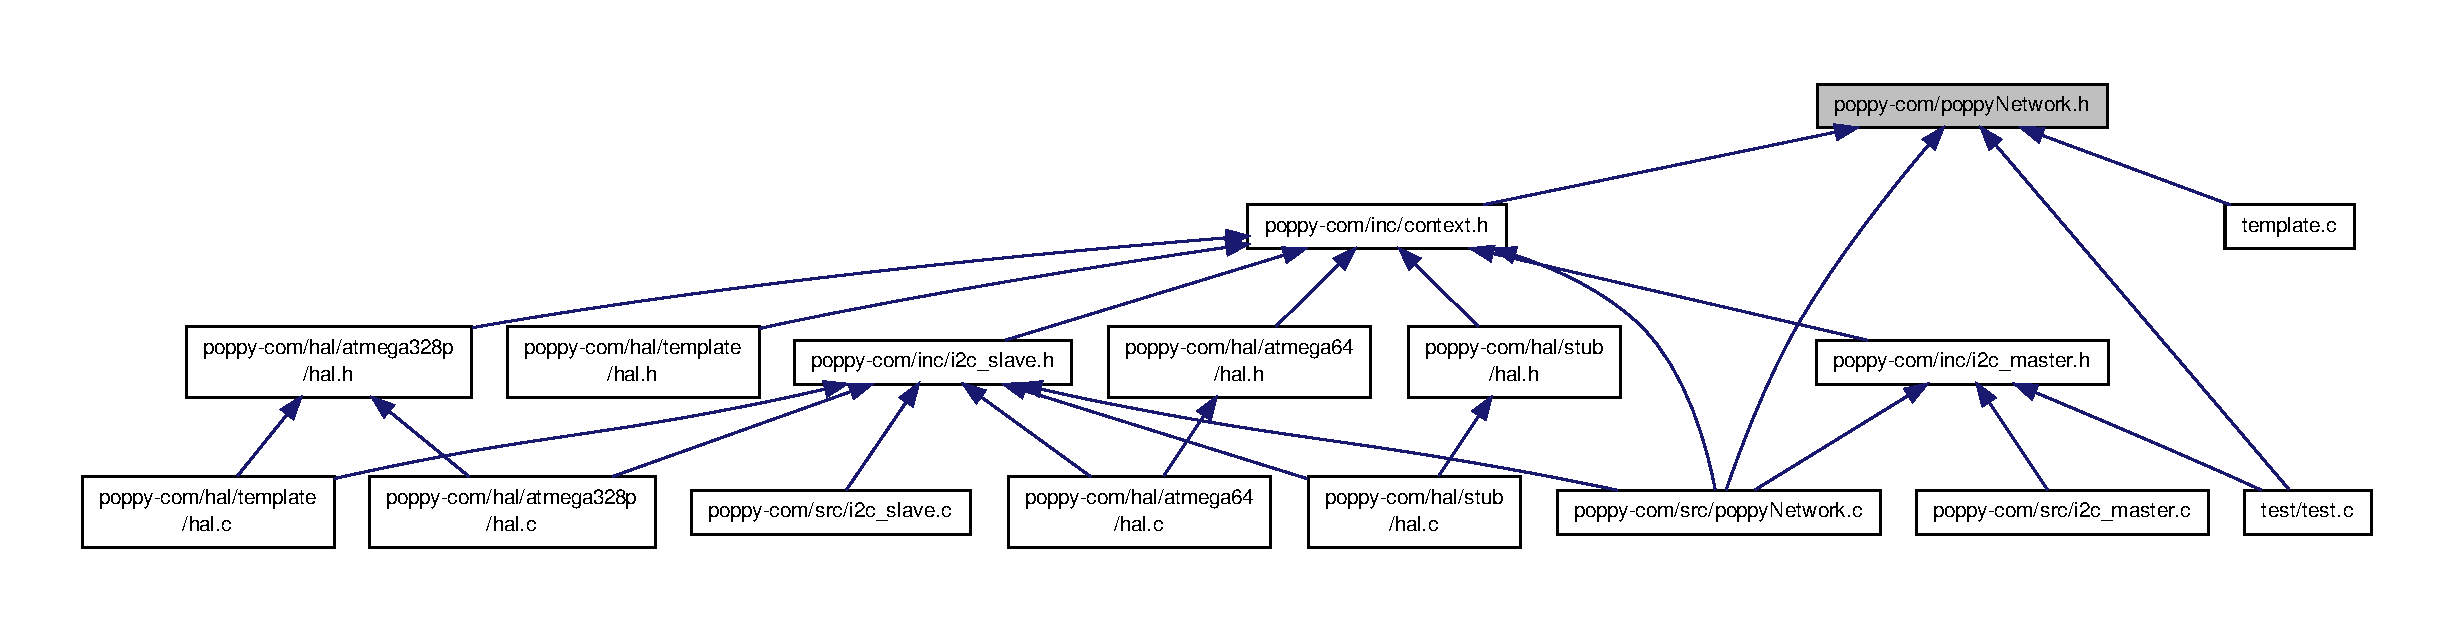
\includegraphics[width=350pt]{poppy_network_8h__dep__incl}
\end{center}
\end{figure}
\subsection*{Classes}
\begin{DoxyCompactItemize}
\item 
struct \hyperlink{structmsg__t}{msg\-\_\-t}
\begin{DoxyCompactList}\small\item\em Message structure. \end{DoxyCompactList}\end{DoxyCompactItemize}
\subsection*{Typedefs}
\begin{DoxyCompactItemize}
\item 
\hypertarget{poppy_network_8h_a4567ad10b049d681c2b327af74719feb}{typedef void($\ast$ {\bfseries R\-X\-\_\-\-C\-B} )(\hyperlink{poppy_network_8h_a1def9945bd875d4a35c81b0c452053d1}{msg\-\_\-dir\-\_\-t} dir, \hyperlink{structmsg__t}{msg\-\_\-t} $\ast$msg)}\label{poppy_network_8h_a4567ad10b049d681c2b327af74719feb}

\item 
\hypertarget{poppy_network_8h_aa4dbf6893d0f30bff45a345c1b4df124}{typedef void($\ast$ {\bfseries T\-X\-\_\-\-C\-B} )(\hyperlink{structmsg__t}{msg\-\_\-t} $\ast$msg)}\label{poppy_network_8h_aa4dbf6893d0f30bff45a345c1b4df124}

\end{DoxyCompactItemize}
\subsection*{Enumerations}
\begin{DoxyCompactItemize}
\item 
enum \hyperlink{poppy_network_8h_a1def9945bd875d4a35c81b0c452053d1}{msg\-\_\-dir\-\_\-t} \{ \hyperlink{poppy_network_8h_a1def9945bd875d4a35c81b0c452053d1a951f819598b53b2729ee0e4c05e6888e}{T\-X}, 
\hyperlink{poppy_network_8h_a1def9945bd875d4a35c81b0c452053d1a4aca20d6e60fffb66e9668b3a6592531}{R\-X}, 
\hyperlink{poppy_network_8h_a1def9945bd875d4a35c81b0c452053d1acb3c9419352b04839e939d4d3f32ce77}{R\-X\-G\-C}, 
\hyperlink{poppy_network_8h_a1def9945bd875d4a35c81b0c452053d1adc6f24fd6915a3f2786a1b7045406924}{E\-N\-D}
 \}
\begin{DoxyCompactList}\small\item\em Message direction enum. \end{DoxyCompactList}\end{DoxyCompactItemize}
\subsection*{Functions}
\begin{DoxyCompactItemize}
\item 
void \hyperlink{poppy_network_8h_ada0ea1c998dbd2179bf435c285d043f0}{poppy\-Network\-\_\-init} (T\-X\-\_\-\-C\-B tx\-\_\-cb, R\-X\-\_\-\-C\-B rx\-\_\-cb, R\-X\-\_\-\-C\-B rxgc\-\_\-cb)
\begin{DoxyCompactList}\small\item\em Initialisation of the Poppy communication lib. \end{DoxyCompactList}\item 
\hypertarget{poppy_network_8h_a7501ac4221ee0c891e53e11e976c6aee}{unsigned char {\bfseries poppy\-Network\-\_\-read} (unsigned char addr, \hyperlink{structmsg__t}{msg\-\_\-t} $\ast$msg, unsigned char reply\-\_\-size)}\label{poppy_network_8h_a7501ac4221ee0c891e53e11e976c6aee}

\item 
unsigned char \hyperlink{poppy_network_8h_a6967645d5bf4139f439a8fa125f2f099}{poppy\-Network\-\_\-write} (unsigned char addr, \hyperlink{structmsg__t}{msg\-\_\-t} $\ast$msg)
\begin{DoxyCompactList}\small\item\em Master mode write function. \end{DoxyCompactList}\end{DoxyCompactItemize}


\subsection{Detailed Description}
Poppy communication main include file. \begin{DoxyAuthor}{Author}
Nicolas Rabault 
\end{DoxyAuthor}
\begin{DoxyVersion}{Version}
0.\-1 
\end{DoxyVersion}
\begin{DoxyDate}{Date}
22 Avril 2015
\end{DoxyDate}
Include this file to use the poppy communication protocole. 

Definition in file \hyperlink{poppy_network_8h_source}{poppy\-Network.\-h}.



\subsection{Enumeration Type Documentation}
\hypertarget{poppy_network_8h_a1def9945bd875d4a35c81b0c452053d1}{\index{poppy\-Network.\-h@{poppy\-Network.\-h}!msg\-\_\-dir\-\_\-t@{msg\-\_\-dir\-\_\-t}}
\index{msg\-\_\-dir\-\_\-t@{msg\-\_\-dir\-\_\-t}!poppyNetwork.h@{poppy\-Network.\-h}}
\subsubsection[{msg\-\_\-dir\-\_\-t}]{\setlength{\rightskip}{0pt plus 5cm}enum {\bf msg\-\_\-dir\-\_\-t}}}\label{poppy_network_8h_a1def9945bd875d4a35c81b0c452053d1}


Message direction enum. 

Module specific register enumerator.

This structure is used to get the message direction but it seems to be useles because we have defferent interrupt for each msg\-\_\-dir case.

This is the minimal include you will need to use poppy-\/com in a module application

This structure is used to list all the specific module register. The first register should be equal to P\-R\-O\-T\-O\-C\-O\-L\-\_\-\-R\-E\-G\-I\-S\-T\-E\-R\-\_\-\-N\-B, because is the first free register. The last register should be M\-O\-D\-U\-L\-E\-\_\-\-R\-E\-G\-I\-S\-T\-E\-R\-\_\-\-N\-B, for the user space register enumerator... \begin{Desc}
\item[Enumerator]\par
\begin{description}
\index{T\-X@{T\-X}!poppy\-Network.\-h@{poppy\-Network.\-h}}\index{poppy\-Network.\-h@{poppy\-Network.\-h}!T\-X@{T\-X}}\item[{\em 
\hypertarget{poppy_network_8h_a1def9945bd875d4a35c81b0c452053d1a951f819598b53b2729ee0e4c05e6888e}{T\-X}\label{poppy_network_8h_a1def9945bd875d4a35c81b0c452053d1a951f819598b53b2729ee0e4c05e6888e}
}]Slave transmiter mode. \index{R\-X@{R\-X}!poppy\-Network.\-h@{poppy\-Network.\-h}}\index{poppy\-Network.\-h@{poppy\-Network.\-h}!R\-X@{R\-X}}\item[{\em 
\hypertarget{poppy_network_8h_a1def9945bd875d4a35c81b0c452053d1a4aca20d6e60fffb66e9668b3a6592531}{R\-X}\label{poppy_network_8h_a1def9945bd875d4a35c81b0c452053d1a4aca20d6e60fffb66e9668b3a6592531}
}]Slave receiver mode. \index{R\-X\-G\-C@{R\-X\-G\-C}!poppy\-Network.\-h@{poppy\-Network.\-h}}\index{poppy\-Network.\-h@{poppy\-Network.\-h}!R\-X\-G\-C@{R\-X\-G\-C}}\item[{\em 
\hypertarget{poppy_network_8h_a1def9945bd875d4a35c81b0c452053d1acb3c9419352b04839e939d4d3f32ce77}{R\-X\-G\-C}\label{poppy_network_8h_a1def9945bd875d4a35c81b0c452053d1acb3c9419352b04839e939d4d3f32ce77}
}]Slave receiver g�n�ral call mode. \index{E\-N\-D@{E\-N\-D}!poppy\-Network.\-h@{poppy\-Network.\-h}}\index{poppy\-Network.\-h@{poppy\-Network.\-h}!E\-N\-D@{E\-N\-D}}\item[{\em 
\hypertarget{poppy_network_8h_a1def9945bd875d4a35c81b0c452053d1adc6f24fd6915a3f2786a1b7045406924}{E\-N\-D}\label{poppy_network_8h_a1def9945bd875d4a35c81b0c452053d1adc6f24fd6915a3f2786a1b7045406924}
}]Slave receiver stop. \end{description}
\end{Desc}


Definition at line 22 of file poppy\-Network.\-h.



\subsection{Function Documentation}
\hypertarget{poppy_network_8h_ada0ea1c998dbd2179bf435c285d043f0}{\index{poppy\-Network.\-h@{poppy\-Network.\-h}!poppy\-Network\-\_\-init@{poppy\-Network\-\_\-init}}
\index{poppy\-Network\-\_\-init@{poppy\-Network\-\_\-init}!poppyNetwork.h@{poppy\-Network.\-h}}
\subsubsection[{poppy\-Network\-\_\-init}]{\setlength{\rightskip}{0pt plus 5cm}void poppy\-Network\-\_\-init (
\begin{DoxyParamCaption}
\item[{T\-X\-\_\-\-C\-B}]{tx\-\_\-cb, }
\item[{R\-X\-\_\-\-C\-B}]{rx\-\_\-cb, }
\item[{R\-X\-\_\-\-C\-B}]{rxgc\-\_\-cb}
\end{DoxyParamCaption}
)}}\label{poppy_network_8h_ada0ea1c998dbd2179bf435c285d043f0}


Initialisation of the Poppy communication lib. 


\begin{DoxyParams}{Parameters}
{\em tx\-\_\-cb} & function pointer into the tx callback. \\
\hline
{\em rx\-\_\-cb} & function pointer into the rx callback. \\
\hline
{\em rxgc\-\_\-cb} & function pointer into the rx general call callback. \\
\hline
\end{DoxyParams}


Definition at line 17 of file poppy\-Network.\-c.

\hypertarget{poppy_network_8h_a6967645d5bf4139f439a8fa125f2f099}{\index{poppy\-Network.\-h@{poppy\-Network.\-h}!poppy\-Network\-\_\-write@{poppy\-Network\-\_\-write}}
\index{poppy\-Network\-\_\-write@{poppy\-Network\-\_\-write}!poppyNetwork.h@{poppy\-Network.\-h}}
\subsubsection[{poppy\-Network\-\_\-write}]{\setlength{\rightskip}{0pt plus 5cm}unsigned char poppy\-Network\-\_\-write (
\begin{DoxyParamCaption}
\item[{unsigned char}]{addr, }
\item[{{\bf msg\-\_\-t} $\ast$}]{msg}
\end{DoxyParamCaption}
)}}\label{poppy_network_8h_a6967645d5bf4139f439a8fa125f2f099}


Master mode write function. 


\begin{DoxyParams}{Parameters}
{\em addr} & Address of the slave. \\
\hline
{\em msg} & Message to send to the slave. \\
\hline
\end{DoxyParams}


Definition at line 85 of file poppy\-Network.\-c.


\hypertarget{template_8c}{\section{template.\-c File Reference}
\label{template_8c}\index{template.\-c@{template.\-c}}
}


Poppy module application side template.  


{\ttfamily \#include \char`\"{}poppy-\/com/poppy\-Network.\-h\char`\"{}}\\*
Include dependency graph for template.\-c\-:
\nopagebreak
\begin{figure}[H]
\begin{center}
\leavevmode
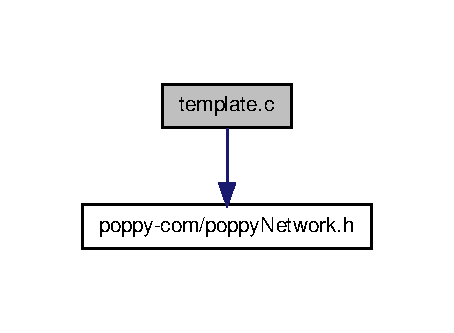
\includegraphics[width=218pt]{template_8c__incl}
\end{center}
\end{figure}
\subsection*{Enumerations}
\begin{DoxyCompactItemize}
\item 
enum {\bfseries module\-\_\-register\-\_\-t} \{ {\bfseries M\-O\-D\-U\-L\-E\-\_\-\-R\-E\-G\-I\-S\-T\-E\-R\-\_\-\-N\-B}, 
{\bfseries T\-E\-S\-T\-\_\-\-R\-E\-G\-I\-S\-T\-E\-R} = P\-R\-O\-T\-O\-C\-O\-L\-\_\-\-R\-E\-G\-I\-S\-T\-E\-R\-\_\-\-N\-B, 
{\bfseries M\-O\-D\-U\-L\-E\-\_\-\-R\-E\-G\-I\-S\-T\-E\-R\-\_\-\-N\-B}
 \}
\end{DoxyCompactItemize}
\subsection*{Functions}
\begin{DoxyCompactItemize}
\item 
\hypertarget{template_8c_ace61de97737b4ab184cc58f6fa90e61b}{void {\bfseries rx\-\_\-cb} (\hyperlink{poppy_network_8h_a1def9945bd875d4a35c81b0c452053d1}{msg\-\_\-dir\-\_\-t} dir, \hyperlink{structmsg__t}{msg\-\_\-t} $\ast$msg)}\label{template_8c_ace61de97737b4ab184cc58f6fa90e61b}

\item 
\hypertarget{template_8c_ab93d299989e0e94c4f6f91d95936a070}{void {\bfseries rxgc\-\_\-cb} (\hyperlink{poppy_network_8h_a1def9945bd875d4a35c81b0c452053d1}{msg\-\_\-dir\-\_\-t} dir, \hyperlink{structmsg__t}{msg\-\_\-t} $\ast$msg)}\label{template_8c_ab93d299989e0e94c4f6f91d95936a070}

\item 
\hypertarget{template_8c_ae4dafcb82441709916a9e68df792f44a}{void {\bfseries tx\-\_\-cb} (\hyperlink{structmsg__t}{msg\-\_\-t} $\ast$msg)}\label{template_8c_ae4dafcb82441709916a9e68df792f44a}

\item 
\hypertarget{template_8c_a840291bc02cba5474a4cb46a9b9566fe}{int {\bfseries main} (void)}\label{template_8c_a840291bc02cba5474a4cb46a9b9566fe}

\end{DoxyCompactItemize}


\subsection{Detailed Description}
Poppy module application side template. \begin{DoxyAuthor}{Author}
Nicolas Rabault 
\end{DoxyAuthor}
\begin{DoxyVersion}{Version}
0.\-1 
\end{DoxyVersion}
\begin{DoxyDate}{Date}
22 Avril 2015
\end{DoxyDate}
Please feel free to copy this template and use it at base for your new Poppy module application. 

Definition in file \hyperlink{template_8c_source}{template.\-c}.


%--- End generated contents ---

% Index
\newpage
\phantomsection
\addcontentsline{toc}{chapter}{Index}
\printindex

\end{document}
